\documentclass{assignment}
\ProjectInfos{光电子技术}{PHYS6651P}{2021-2022学年第一学期}{第六章作业}{}{陈稼霖}[https://github.com/Chen-Jialin]{SA21038052}

\begin{document}
\begin{prob}
    梯度折射率光纤的折射率分布满足 $n^2(r)=n^2(0)(1-\alpha^2r^2)$,其中 $\alpha=140\text{rad}\cdot\text{mm}^{-1}$,试求当近轴光线入射时,光纤中光线每传播一周期的的长度 $L$?
\end{prob}
\begin{sol}
    光纤折射率分布为
    \begin{gather}
        n(r)=n(0)\sqrt{1-\alpha^2r^2}\approx n(0)\left(1-\frac{1}{2}\alpha^2r^2\right)=n(0)\left(1-\frac{1}{2}Ar^2\right),\\
        \Longrightarrow A=\alpha^2.
    \end{gather}
    当近轴光线入射时, 光纤中光线每传播一周期的长度为
    \begin{align}
        L=\frac{2\pi}{\sqrt{A}}=\frac{2\pi}{\alpha}=0.0449\text{ mm}=44.9\,\mu\text{m}.
    \end{align}
\end{sol}

\begin{prob}
    已知自聚焦棒轴线折射率 $1.5$,周期 $48$ mm,用它制造超短焦距透镜作光栅耦合器,求该自聚焦透镜的长度和焦距.
\end{prob}
\begin{sol}
    自聚焦棒折射率分布为
    \begin{align}
        n(r)=n(0)\left(1-\frac{1}{2}Ar^2\right),
    \end{align}
    其中轴线折射率 $n(0)=1.5$,
    \begin{align}
        A=\left(\frac{2\pi}{L}\right)^2=0.171\text{ mm}^{-2}.
    \end{align}
    该自聚焦透镜的长度为
    \begin{align}
        z=\frac{L}{4}=12\text{ mm},
    \end{align}
    焦距为
    \begin{align}
        f=\frac{1}{n_0\sqrt{A}}=\frac{L}{2\pi n_0}=5.09\text{ mm}.
    \end{align}
\end{sol}

\begin{prob}
    在弱传导近似下,利用公式(5.97)计算 EH$_{11}$ 模和 HE$_{31}$ 模的截止条件,并利用标量模理论解释其物理原因.
\end{prob}
\begin{sol}
    利用公式
    \begin{align}
        \frac{(m-1)J_{m-1}(U)}{U}=\frac{1}{2}(J_{m-2}(U)+J_n(U))
    \end{align}
    可将式 (5.97)
    \begin{align}
        \left[\left(\frac{n_1}{n_2}\right)^2+1\right]J_{m-1}(U)=\frac{U}{m-1}J_m(U)
    \end{align}
    化简为
    \begin{align}
        \frac{J_{m-2}(U)}{J_m(U)}=\frac{n_2^2-n_1^2}{n_2^2+n_1^2}.
    \end{align}
    在弱导条件下, $n_1\approx n_2$, 有
    \begin{align}
        J_2(U)=0.
    \end{align}
    对 $H$
\end{sol}

\begin{prob}
    如果在 $\frac{1}{4}$ 拍长的两个自聚焦透镜对之间的准直光路中插入法拉第旋光器和两个偏振器,就可以做成光纤隔离器,如下图所示,简要说明其原理.
    \begin{figure}[h]
        \centering
        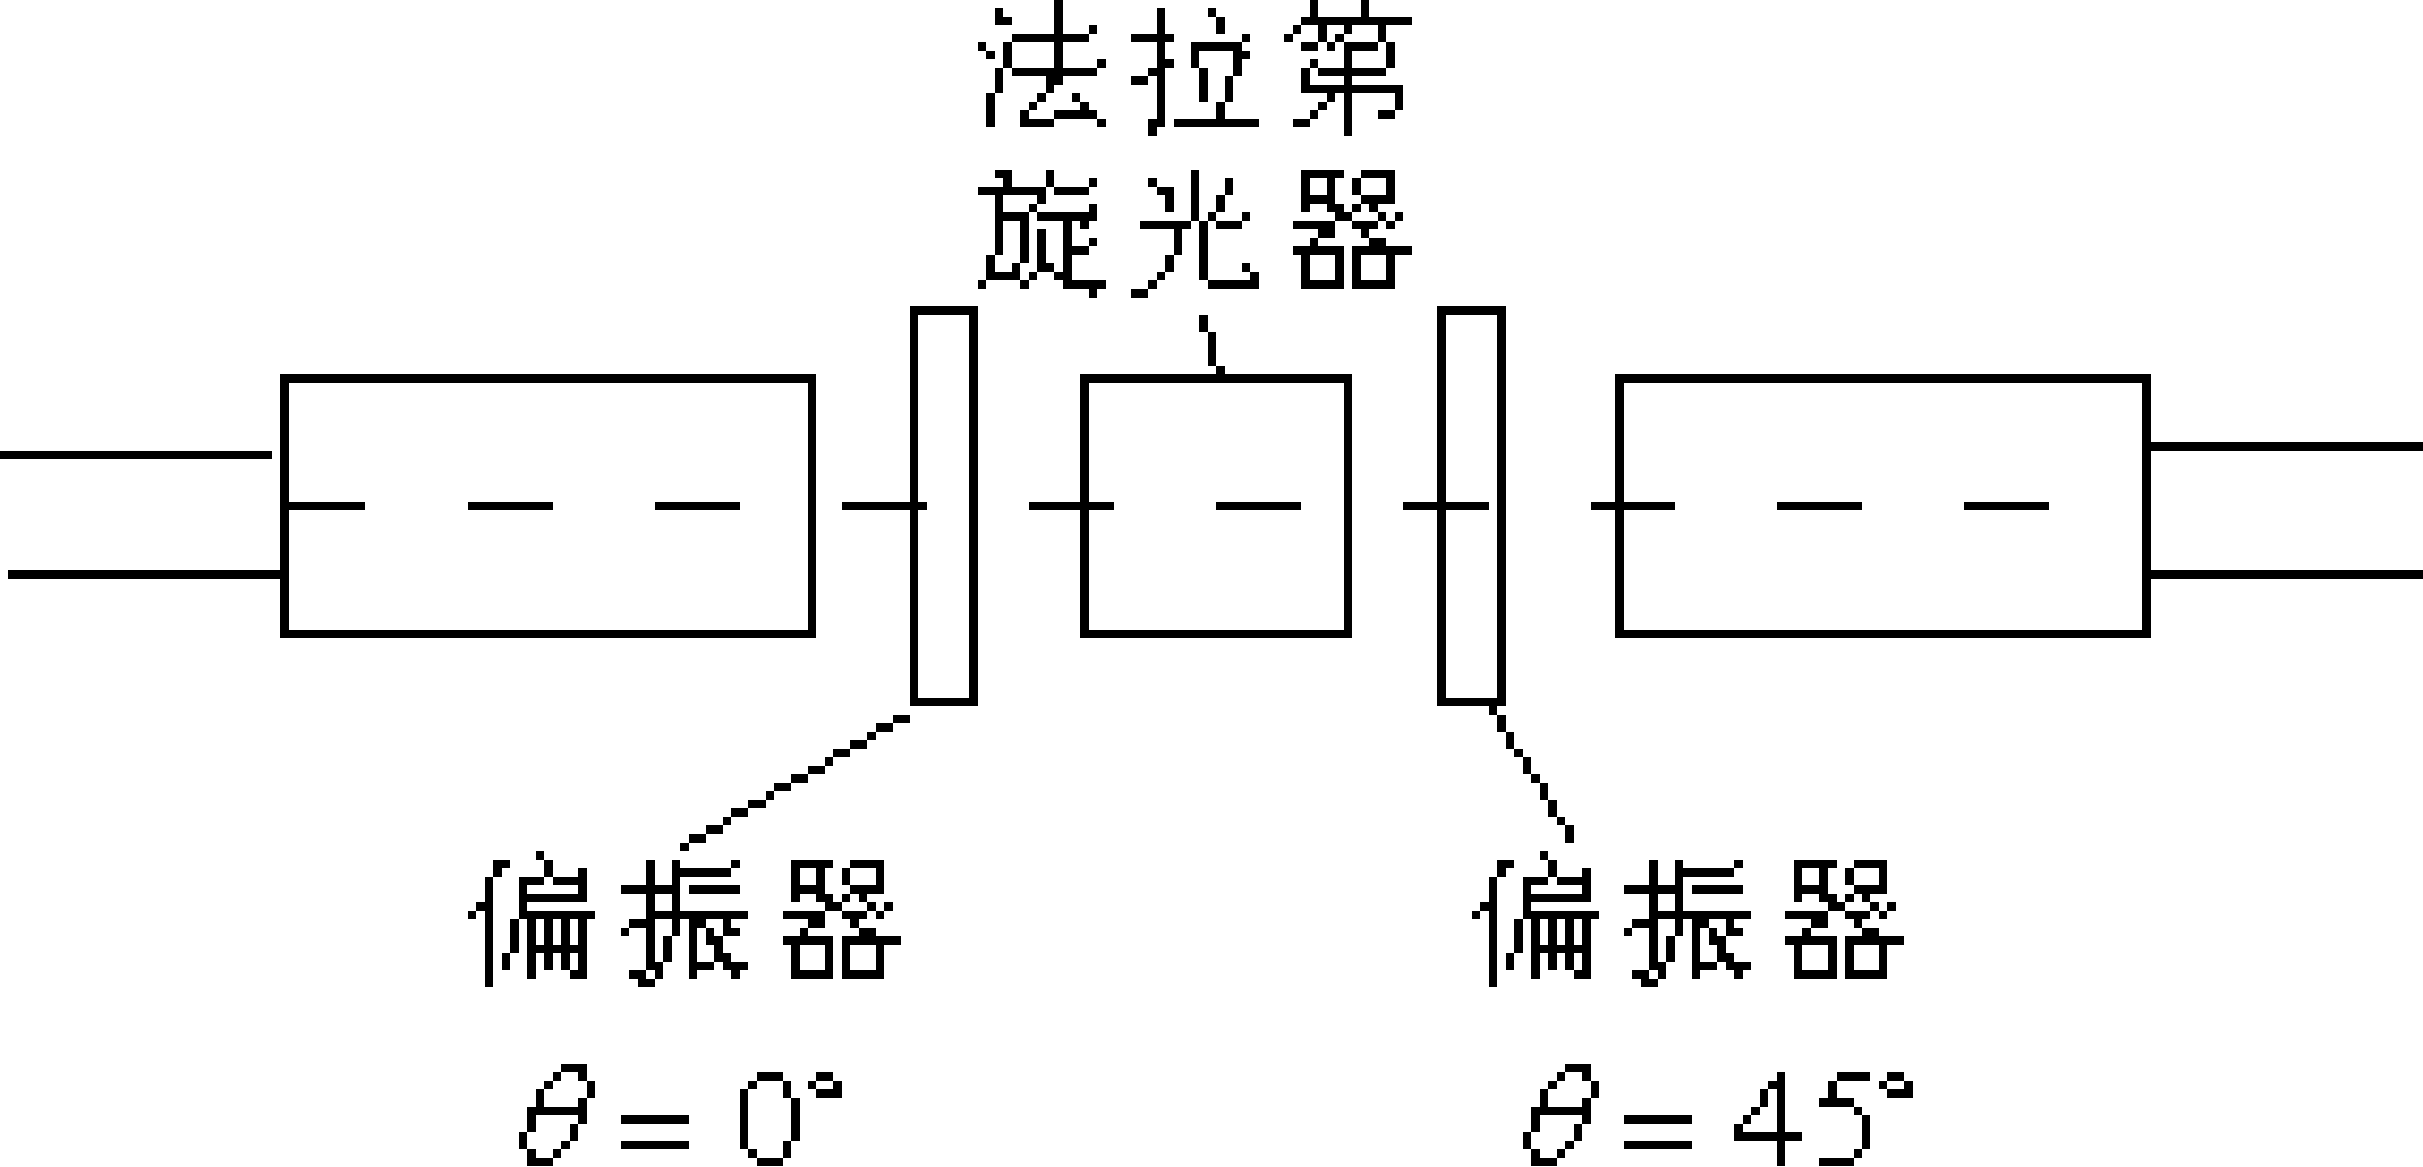
\includegraphics[width=.5\columnwidth]{2-4.png}
    \end{figure}
\end{prob}
\begin{ans}
    当光从左侧入射, 经过自聚焦透镜后变成大致平行的光, 经 $\theta=0^{\circ}$ 的偏振器后只剩下沿垂直方向偏振的光, 垂直偏振光经过法拉第旋光器后偏振变成与垂直方向成 $45^{\circ}$ 角, 因此可以通过 $\theta=45^{\circ}$ 的偏振器, 进而经过自聚焦透镜后耦合进入右侧的光纤.

    当光从右侧入射, 经过自聚焦透镜后变成大致平行的光, 经 $\theta=45^{\circ}$ 的偏振器后只剩下偏振与垂直方向成 $45^{\circ}$ 角的光, 再经过法拉第旋光器后变成水平偏振光, 无法通过 $\theta=0^{\circ}$ 的偏振器.

    因此, 该结构可以保证光的单向传播, 即实现了光纤隔离器的功能.
\end{ans}
\end{document}